% !TeX spellcheck = cs_CZ
%---------------------------------------------------------------------------------------------------
% mai2ch01.tex
%---------------------------------------------------------------------------------------------------
\setchaptertoc
\chapter{Vícerozměrná linearita aneb lineární algebra podruhé}\label{mai:IIchapI}

  V kapitole \ref{mai:IchapII} dílu \ref{part:MAI} jsme se seznámili s elegantní dámou lineární
  algebrou. Pomocí jejích pravidel jsme nejen řešili soustavy lineárních rovnic, ale také počítali s
  maticemi a vektory. Zatímco operace s maticemi, a koneckonců i řešení lineárních rovnic pomocí
  matic bychom mohli chápat jako užitečnou ekvilibristiku s číselnými soubory, za počítáním s
  vektory se zdálo být přece jen něco hlubšího a závažnějšího. Vázané vektory pro nás totiž byly
  orientovanými úsečkami v trojrozměrném euklidovském prostoru, v němž bylo definováno měření délek
  a úhlů. Volné vektory pak byly množinami stejně velkých a souhlasně rovnoběžných orientovaných
  úseček. Jednalo se tedy o \emph{geometrické objekty}. Každý vektor byl určen svou velikostí a
  směrem. Směr byl přitom zadán například pomocí úhlů mezi daným vektorem a vybranými směry, které
  byly předem pevně zvoleny. Mohli jsme s vektory provádět základní algebraické operace, jimiž jsou
  sčítání vektorů a násobení vektoru číslem, podle pravidel zavedených pro (v tomto případě řádkové)
  matice. S vektory v trojrozměrném prostoru jsme mohli velmi pohodlně počítat jako s trojicemi
  čísel. Na druhé straně jsme vektory vyjadřovali jako lineární kombinace jiných vektorů, tvořících
  v prostoru všech vektorů \emph{bázi}. Koeficienty lineární kombinace, která představovala zápis
  daného vektoru ve zvolené bázi, byly jeho \emph{složkami} v této bázi. Při změně báze se změnily
  složky vektoru, vektor sám však nikoliv. Vektor je stále sám sebou, jen se v různých bázích jinak
  tváří - projeví se jinou trojicí čísel. Protože se však při změně báze změní složky vektoru přesně
  definovaným způsobem (vzpomeňte na transformační vztahy), dokážeme jej vždy rozpoznat. Tuto
  vlastnost, \emph{invarianci vůči volbě báze}, mají všechny geometrické objekty. A je to právě
  algebra, která nám umožňuje tyto objekty reprezentovat číselnými soubory a také tak s nimi
  počítat. Jde-li navíc o objekty řídící se lineárními pravidly. jakými jsou například distributivní
  zákony, je počítání s nimi, v rámci \emph{lineární algebry}, zvláště jednoduché. Oceníme to
  zejména v prostorech vyšší dimenze, než je náš běžný euklidovský prostor. Při počítání s vektory v
  trojrozměrném prostoru, kde umíme měřit délky a úhly a kde platí trigonometrická pravidla, bychom
  se bez rutinních algebraických procedur ještě třeba obešli. Už ale například ve čtyřrozměrném
  časoprostoru, v němž se odehrávají všechny přírodní jevy a v němž je třeba formulovat fyzikální
  zákony, však pro měření délek a úhlů platí jiná pravidla, než jsou obvyklá v běžném, tj.
  trojrozměrném euklidovském, prostoru. Například tam neplatí čtyřrozměrná verze Pythagorovy věty. A
  někdy je příroda dokonce tak nepřívětivá, že nás nutí pracovat i s prostory vícerozměrnými.
  Například jedna z velmi účinných teorií pro výklad chování elementárních částic, teorie strum, je
  založena na geometrii prostoru jedenáctirozměrného. A v takových dimenzích jsme už s jakkoli
  vynikající geometrickou představivostí v koncích. Tehdy se vděčně obracíme k metodám algebry. V
  této kapitole, jak její název napovídá, půjde o algebru lineární
  
  \section{Prostory s vektory}
    V kapitole \ref{mai:IchapII} jsme pracovali s číselnými maticemi typu \(m/n\), tj. soubory 
    čísel uspořádaných v \(m\) řádcích a \(n\) sloupcích, a zavedli jsme pro ně operaci součtu a 
    násobení číslem. Zjistili jsme, že pro sčítání matic a násobení matice číslem platí určitá 
    pravidla. (Jejich souhrn je uveden v samém závěru odstavce \ref{mai:IchapIIsecIIIsubIII}. V 
    odstavci \ref{mai:IchapIIsecIV} jsme zase počítali s vektory. Ty měly jednou \emph{konkrétní 
    podobu} řádkových matic s pravidly pro jejich sčítání a násobení číslem, podruhé, v 
    trojrozměrném prostoru, naopak \emph{konkrétní podobu} orientovaných úseček, resp. množin, 
    které byly orientovanými úsečkami vytvořeny, generovány. Zavedli jsme tenkrát konkrétní způsob 
    sčítání vektorů a násobení vektoru číslem pomocí geometrických operací. Součet dvou vektorů 
    \(\vec{u}\) a \(\vec{v}\) znamenal, že jsme podle zcela určitého pravidla, pravidla 
    vektorového rovnoběžníka přiřadili uspořádané dvojici \([\vec{u},\vec{v}]\) třetí vektor 
    \(\vec{u} + \vec{v}\), násobek vektoru a čísla byl opět vektor \(\alpha\vec{u}\), který jsme 
    přiřadili dvojici \([\alpha,\vec{u}]\) tvořené číslem a vektorem. Uvedli jsem, že pravidla pro 
    tyto \emph{geometrické} operace jsou shodná s pravidly pro počítání s maticemi a lze je dokázat 
    i geometrickými postupy. Množinu volných vektorů generovaných orientovanými úsečkami spolu s 
    uvedenými dvěma operacemi jsme nazvali \textbf{vektorovým prostorem}. Šlo tedy o zcela odlišné 
    množiny základních objektů a zcela odlišným způsobem definované operace, pro které se však dala 
    dokázat tatáž pravidla. Nyní se podíváme na problém definice vektorového prostoru obecněji a 
    poněkud \uv{opačně}. Budeme pracovat s \emph{nosnou množinou} \(V\), a přitom nebude podstatné, 
    jak konkrétně vypadají její prvky. Ani je nebudeme označovat šipkami (u šipek ze zvyku 
    zůstaneme pouze v případě orientovaných úseček v \(\mathbb{R}^1\), \(\mathbb{R}^2\) a 
    \(\mathbb{R}^3\), nebo vektorů s fyzikálním významem). Dále přibereme do hry množinu všech 
    komplexních čísel \(\mathbb{C}\), popřípadě jen množinu všech reálných čísel \(\mathbb{R}\) a 
    definujeme dvě operace (\emph{zobrazení}):
    \begin{subequations}\label{mai:eq046}
      \begin{align}
        V \times V \ni [a,b]            &\longrightarrow c\in V, \label{mai:eq046a}  \\
        \mathbb{C}\times V\ni[\alpha,a] &\longrightarrow d\in V. \label{mai:eq046b}
      \end{align}
    \end{subequations}
    Prvek \(c\) nazýváme \emph{součet} prvků \(a\) a \(b\) a značíme jej \(c = a + b\) prvek \(d\) 
    je \(\alpha\)-\emph{násobek} prvku \(a\) a značíme \(d = \alpha a\). Zobrazení uvedená ve 
    vztazích (\ref{mai:eq046}) však nebudou moci být úplně libovolná. Budeme požadovat, aby měla 
    určité vlastnosti, konkrétně ty, které jsou uvedeny pro matice na konci odstavce 
    \ref{mai:IchapIIsecIIIsubIII}. Teprve pak řekneme, že množina \(V\) spolu s operacemi 
    (\ref{mai:eq046}) splňujícími potřebné požadavky je vektorovým prostorem. Vidíme, že takto naše 
    uvažování výrazně posuneme na abstraktní úroveň. Bude lhostejné, co jsou prvky nosné množiny, 
    bude nepodstatné, jak konkrétně jsou definovány operace sčítání prvků a násobení prvku číslem. 
    Důležité bude jen to, aby abstraktní operace s abstraktními prvky splňovaly konkrétní pravidla. 
    Než však k definici vektorového prostoru přistoupíme, všimneme si ještě některých jiných 
    struktur s jednou nebo dvěma operacemi, které samy do oblasti lineární algebry nepatří, ale 
    mohou být užitečné pro definici vektorového prostoru, popřípadě mají významné fyzikální 
    aplikace.
      
      \subsection{Algebraické struktury s jednou operací, hlavně grupy}
        Při zavádění operací s vektory jsme zcela automaticky využívali toho, že umíme počítat s 
        reálnými, popřípadě i s komplexními čísly. Skutečnost, že čísla umíme sčítat, násobit a 
        provádět s nimi řadu dalších operací, považujeme za tak přirozenou a samozřejmou, že nad ní 
        vůbec nepřemýšlíme. Již samotné operace sčítání a násobení vytvářejí na množině čísel velmi 
        bohatou \textbf{algebraickou strukturu}. Tento pojem si nyní přiblížíme. 
        
        Algebraickou strukturu s jednou operací získáme, vezmeme-li v úvahu první ze zobrazení 
        (\ref{mai:eq046}), nosnou množinu označíme tentokrát podle zvyku \(G\):
        \begin{subequations}\label{mai:eq047}
          \begin{align}
            G \times G \ni [a,b] &\longrightarrow a + b \in G,                  \label{mai:eq047a}\\
            G \times G \ni [a,b] &\longrightarrow a \cdot b \in G.              \label{mai:eq047b}
          \end{align}
        \end{subequations}
        Pokud použijeme první možnosti označení této operace, hovoříme o operaci \emph{sčítání} a 
        \emph{aditivní} struktuře, v případě druhé možnosti o operaci \emph{násobení} a 
        \emph{multiplikativní} struktuře. Toto terminologické rozlišení nemá obecně žádný hlubší 
        význam. Je spíše otázkou zvyklosti a souvisí především s algebraickou strukturou číselných 
        množin, kterou běžně používáme, aniž o ní přemýšlíme (čísla sčítá a násobí školák, 
        obchodník i účetní a o nějaké abstraktní struktuře nic netuší).
        
        Zobrazení (\ref{mai:eq047}) samo o sobě, aniž na ně klademe další požadavky (podstatné je 
        pouze to, že dvěma prvkům nosné množiny přiřadí prvek \emph{téže množiny}), definuje 
        nejjednodušší algebraickou strukturu s jednou operací, zvanou \textbf{grupoid}. Grupoid 
        není pro fyzikální aplikace příliš užitečný, ale je základem pro konstrukci zajímavějších a 
        užitečnějších struktur. Přidáme-li k definici grupoidu požadavek \emph{asociativity} 
        zobrazení \(G \times G \ni [a, b] \longrightarrow a + b \in G\) (nebo \(G \times G \ni [a, 
        b] \longrightarrow a \cdot b \in G\))
        \begin{subequations}\label{mai:eq048}
          \begin{align}
            (a+b) + c          &= a + (b + c),                                  \label{mai:eq048a}\\
            (a\cdot b) \cdot c &= a \cdot (b \cdot c)                           \label{mai:eq048b} 
          \end{align}
        \end{subequations}
        pro libovolné prvky \(a, b, c \in G\), stane se množina \(G\) spolu s operací „\(+\)“, nebo 
        „-“ \textbf{pologrupou}. I pologrupa je z hlediska fyzikálních aplikací poněkud chudá, 
        další požadavek na zobrazení (\ref{mai:eq047}) z ní však již učiní strukturu v matematice i 
        fyzice nepostradatelnou, grupu. Pologrupa, ve které existuje prvek \(0_G\in G\) a současně 
        ke každému prvku \(a \in G\) existuje prvek \((-a) \in G\) tak, že platí
        \begin{subequations}\label{mai:eq049}
          \begin{align}
            a + 0_G  &= 0_G + a = a,                                            \label{mai:eq049a}\\ 
            a + (-a) &= (-a) + a = 0_G,                                         \label{mai:eq049b}
          \end{align}
        \end{subequations}
        se nazývá \textbf{aditivní grupou}. Prvek \(0_G\) je univerzální pro celou grupu (žádný 
        jiný s touto vlastností v grupě \(G\) není) a nazývá se \emph{neutrální prvek grupy} neboli 
        \textbf{nula}, prvek \((-a)\) je \textbf{opačný} k prvku \(a\). Pro dané \(a\) je určen 
        jednoznačně. V případě operace násobení mají vlastnosti \ref{mai:eq049} tvar
        \begin{subequations}\label{mai:eq050}
          \begin{align}
            a \cdot e_G    &= e_G    \cdot a = a,                       \label{mai:eq050a}\\
            a \cdot a^{-1} &= a^{-1} \cdot a = e_G,                     \label{mai:eq050b}
          \end{align}
        \end{subequations}
        a \(G\) se nazývá \textbf{multiplikativní grupou}. Prvek \(e_G\) je opět univerzální pro 
        celou grupu a nazývá se \textbf{neutrální} prvek grupy, neboli \emph{jednička}, prvek 
        \(a^{-1}\) je \textbf{inverzní} k prvku \(a\).
        
        Každá operace \ref{mai:eq047} v množině \(G\), která splňuje vztahy asociativity 
        \ref{mai:eq048} a vztahy specifikující nulu a opačný prvek, nebo jedničku a inverzní prvek 
        typu \ref{mai:eq049}, nebo \ref{mai:eq050}, představuje \emph{grupovou operaci} bez ohledu 
        na to, podobá-li se spíše sčítání, nebo spíše násobení, či dokonce něčemu jinému, například 
        skládání zobrazení. Má-li grupa konečný počet prvků, nazývá se tento počet jejím 
        \emph{řádem}.

        %---------------------------------------------------------------
        % !TeX spellcheck = cs_CZ
\wikitextrule
\begin{example}\label{mai:exam046}
  \textbf{Kolik nul má (aditivní) grupa?}\newline\small
  Jak dokážeme, že má grupa právě jednu nulu? Co když předchozímu tvrzení nebudeme věřit? Můžeme se 
  o jeho pravdivosti přesvědčit? Ten, kdo mu nevěří, si může třeba představit, že grupa má nuly 
  dvě. Označme je \(0_G\) a \(\overline{0}_G\). Vztah \ref{mai:eq049} platí pro libovolný prvek 
  grupy, proto \(0_G + \overline{0}_G = 0_G\) (to jsme brali \(a = 0_G\) a \(\overline{0}_G\) 
  považovali za nulu) a současně \(0_G + \overline{0}_G = \overline{0}_G\) (nyní zase byl prvek 
  \(0_G\) v roli nuly a \(a = \overline{0}_G\)). Je vidět, že \(0_G = \overline{0}_G\). Nula je 
  tedy skutečně jen jedna. Podobnou úvahu můžeme provést pro jedničku multiplikativní grupy. Platí 
  tedy tvrzení:
  
  \noindent
  \adjustbox{}{Neutrální prvek grupy je určen jednoznačně.}

  
  Stejně tak bychom mohli mít pochybnosti o tom, že opačný prvek k danému \(a\in G\) je jen jeden. 
  Předpokládejme, že \(b\) a \(c\) jsou dva opačné prvky k \(a\). Platí \(a + b = 0_G\). Přičteme k 
  této rovnosti \(c\) zleva, tj. \(c + a + b = c\). Protože však \(c + a = 0_G\), dostáváme \(b=c\) 
  a tedy:
 
  \noindent
  \adjustbox{}{Opačný (resp. inverzní) prvek k libovolně zvolenému prvku grupy je určen 
  jednoznačně.}
  \normalsize
\end{example}
        %---------------------------------------------------------------
        
        V úvodu odstavce jsme se zmínili o tom, že množiny reálných a komplexních čísel získají 
        zavedením běžných operací sčítání a násobení jistou algebraickou strukturu. Všimněme si 
        jich nyní podrobněji. 
        
        %---------------------------------------------------------------
        % !TeX spellcheck = cs_CZ
\wikitextrule
\begin{example}\label{mai:exam047}
  \textbf{Algebraická struktura a kupecké počty}\newline\small
    Uvažujme o množině reálných čísel \(G = \mathbb{R}\) tak, jako bychom je uměli jen 
    sčítat. Násobení si zatím nevšímejme. Sčítání reálných čísel je zobrazení typu prvního 
    vztahu v \ref{mai:eq047}, které bezpochyby splňuje požadavky \ref{mai:eq048} a 
    \ref{mai:eq049}. Neutrálním prvkem \(0_\mathbb{R}\) je \uv{obyčejná} nula, opačným prvkem k 
    číslu \(a\) je \(-a\), položené na reálné ose symetricky k \(a\) vzhledem k nule. Množina 
    reálných čísel s operací sčítání je tedy aditivní grupou. Pro operaci sčítání dokonce platí 
    něco navíc - komutativní zákon
    \begin{equation}\label{mai:eq051}
      a + b = b + a \qquad\text{pro libovolné}\qquad a,b\in\mathbb{R}.
    \end{equation} 
    Grupu s komutativním zákonem nazýváme grupou \emph{komutativní} nebo také \textbf{abelovskou}.
    
      \adjustbox{}{Množina reálných čísel s operací sčítání je komutativní grupou.}
    
    Nyní se místo na sčítání zaměřme na násobení reálných čísel a znovu posuďme vlastnosti grupy. 
    Násobení reálných čísel je zobrazením typu druhého vztahu v \ref{mai:eq047} a splňuje požadavek 
    asociativnosti \ref{mai:eq048}. Dále je zřejmé, že číslo \(e_\mathbb{R}\) (\uv{obyčejná} 
    jednička) vyhovuje prvnímu požadavku ve vztazích \ref{mai:eq050}. Potíž je s požadavkem druhým. 
    Inverzní prvek najdeme jen k nenulovým číslům. Nula inverzní prvek nemá. Tato zdánlivá drobnost 
    je příčinou toho, že \textbf{množina reálných čísel s operací násobení není grupou}.
  \normalsize
\end{example}
        %---------------------------------------------------------------
        
        %---------------------------------------------------------------
        % !TeX spellcheck = cs_CZ
\wikitextrule
\begin{example}\label{mai:exam048}
  \textbf{Algebraická struktura na množině komplexních čísel}\newline\small
    Množina \(\cmplxset\) komplexních čísel je kartézským součinem reálných os, \(\cmplxset = 
    \mathbb{R} \times \mathbb{R}\), tedy množinou uspořádaných dvojic \([a, b]\) čísel reálných. 
    Značíme \(z = [a, b]\). Reálné číslo \(a = \operatorname{Re}(z)\) je \emph{reálnou} částí 
    komplexního čísla \(z\) a reálné číslo \(b = \operatorname{Im}(z)\) částí \emph{imaginární}. 
    Operace sčítání a násobení komplexních čísel jsou definovány takto:
    \begin{align*}
      \cmplxset\times\cmplxset\ni\left[[a_1, b_1],[a_2, b_2]\right] &\longrightarrow
        [a_1, b_1] + [a_2, b_2] = [a_1 + a_2, b_1 + b_2]\in\cmplxset,                   \\
      \cmplxset\times\cmplxset\ni\left[[a_1, b_1],[a_2, b_2]\right] &\longrightarrow
        [a_1, b_1] \cdot [a_2, b_2] = 
        [a_1 \cdot a_2 - b_1 \cdot b_2, a_1 \cdot b_2 + a_2 \cdot b_1]\in\cmplxset.
    \end{align*}
    
    \adjustbox{}{Množina komplexních čísel s operací součtu je komutativní grupou.}
    
    Jejím neutrálním prvkem je číslo \(0_\cmplxset = [0,0]\), opačným prvkem k číslu \(z = [a, b]\) 
    je \(-z = [-a, - b]\). Při operaci násobení je neutrálním prvkem číslo [1,0], prvkem inverzním 
    k číslu \(z = [a, b] \neq 0_\cmplxset\) je
    \begin{equation*}
      z^{-1} = \left[\dfrac{a}{a^2 + b^2}, \dfrac{-b}{a^2 + b^2}\right].
    \end{equation*}
    
    K číslu \(0_\cmplxset = [0,0]\) však inverzní prvek opět neexistuje. Množina komplexních čísel 
    \textbf{není grupou vzhledem k násobení}.
  \normalsize
\end{example}
        %---------------------------------------------------------------
        
        O podmnožině \(H \subset C\) grupy \(G\) s operací sčítání nebo násobení zúženou na \(H\), 
        která je sama grupou, hovoříme jako o \textbf{podgrupě} grupy \(G\). Například množina 
        reálných čísel zapsaných ve tvaru \(z = [a, 0]\) se sčítáním je podgrupou množiny 
        komplexních čísel. Koho grupy nebaví a chce se rychle prokousat k vektorovým prostorům, 
        které jsou koneckonců hlavní náplní našeho příběhu o lineární algebře, může zbytek tohoto 
        odstavce přeskočit. Ale byla by to škoda, grupy jsou opravdu zajímavé.

        %---------------------------------------------------------------
        % !TeX spellcheck = cs_CZ
\wikitextrule
\begin{example}\label{mai:exam050}
  \textbf{Struktura aditivní grupy na podmnožinách reálné osy}\newline\small

  \normalsize
\end{example}
        %---------------------------------------------------------------
        
        %---------------------------------------------------------------
        % !TeX spellcheck = cs_CZ
\wikitextrule
\begin{example}\label{mai:exam050}
  \textbf{Grupy některých číselných objektů}\newline\small

  \normalsize
\end{example}
        %---------------------------------------------------------------

        %---------------------------------------------------------------
        % !TeX spellcheck = cs_CZ
\wikitextrule
\begin{example}\label{mai:exam051}
  \textbf{Grupy nemusí být tvořeny jen čísly}\newline\small
  {\centering
    \captionsetup{type=figure}
    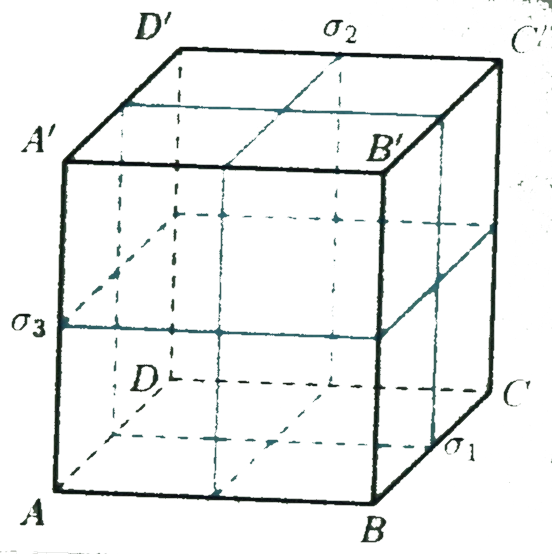
\includegraphics[width=0.4\linewidth]{mai_fig037.png}
    \captionof{figure}{Zadáni přímky. \cite[s.~6]{Musilova2012MA2}
    \label{mai:fig000}}
    \par}
  \normalsize
\end{example}
        %---------------------------------------------------------------
        
      \subsection{Algebraické struktury se dvěma operacemi, hlavně pole}
      
      \subsection{Co je to vektorový prostor?}
        %---------------------------------------------------------------
        % !TeX spellcheck = cs_CZ
\begin{mdframed}[style=mdexam]
  \begin{example}\label{mai:exam107}
    \textbf{Uspořádané \(n\)-tice komplexních čísel jako vektory}\newline
    Na množině uspořádaných \(n\)-tic komplexních čísel
    \begin{equation*}
      a=(\alpha^1,\alpha^2,\ldots,\alpha^n)\in\cmplxset\times\cmplxset\times\cdots\times\cmplxset
    \end{equation*}
    zavedeme operace sčítání
    \begin{align}
      a + b &= (\alpha^1,\alpha^2,\ldots,\alpha^n) + (\beta^1,\beta^2,\ldots,\beta^n)   \nonumber\\
            &= (\alpha^1+ \beta^1,\alpha^2 +\beta^2,\ldots,\alpha^n + \beta^n)    \label{mai:eq098}
    \end{align}
    a násobení skalárem (komplexním číslem)
    \begin{equation}\label{mai:eq099}
      \gamma a = \gamma(\alpha^1,\alpha^2,\ldots,\alpha^n) 
               = (\gamma\alpha^1,\gamma\alpha^2,\ldots,\gamma\alpha^n). 
    \end{equation}
    O tom, že takto konkrétně definované operace splňují všechny axiomy vektorového prostoru nad
    polem komplexních čísel, se snadno přesvědčíme sami. Jde nyní o to, zda se jedná o prostor
    konečné dimenze a jaká tato dimenze je. Označme
    \begingroup
    \setlength{\arraycolsep}{0pt}
    \begin{equation*}
    \begin{array}{rl}
      % https://tex.stackexchange.com/questions/114959/putting-row-of-dots-in-an-equation
      e_1     &= (1, 0, 0, \ldots, 0, 0),  \\
      e_2     &= (0, 1, 0, \ldots, 0, 0),  \\
      \hdotsfor{2}                         \\
      e_{n-1} &= (0, 0, 0, \ldots, 1, 0),  \\
      e_n     &= (0, 0, 0, \ldots, 0, 1).
    \end{array}
    \end{equation*}
    Tyto \(n\)-tice jsou lineárně nezávislé. Zkusme z nich udělat nulovou lineární kombinaci!
    \begin{align*}
      \gamma^1e_1 + \gamma^2e_2 + \cdots + \gamma^ne_n 
        &= (\gamma^1, \gamma^2, \ldots, \gamma^n)              \\
        &= (0,0, \ldots, 0).
    \end{align*}
    Je zřejmé, že všechny koeficienty \(\gamma^j, j\in\{1,2,\ldots,n\}\), jsou nulové \(n\)-tice
    \(e_1\) až \(e_n\) jsou tedy lineárně nezávislé. Zvolíme-li libovolnou \(n\)-tici
    \(\alpha=(\alpha^1, \alpha^2,\ldots, \alpha^n\), můžeme ji zapsat ve tvaru
    \begin{equation*}
      a = \alpha^1e_1 + \alpha^2e_2 + \ldots + \alpha^ne_n.
    \end{equation*}
    Soubor \(e_1, e_2, \ldots, e_n\) je tedy bází ve vektorovém prostoru uspořádáných \(n\)-tic nad
    polem komplexních čísel. Tento prostor je \(n\)-rozměrný. Báze, kterou jsme nalezli, je
    obzvlášťě jednoduchá, a proto je čsto používána. Říkáme jí báze \emph{standardní}. Podobně
    bychom mohli zkonstruovat standrardní bázi vektorovém prostoru \(n\)-tic reálných čísel nad
    polem \(\realset\) \cite[s.~27]{Musilova2012MA2}.
    \endgroup
  \end{example}
\end{mdframed}
        %---------------------------------------------------------------
  \section{Lineární zobrazení vektorových prostorů}
  \section{Vektorové prostory se skalárním součinem}
    \subsection{Ortogonální doplňky}
      Nechť \(U\) je podprostor vektorového prostoru \(V\). Ortogonální doplněk $U^\bot$ obsahuje 
      všechny vektory, které jsou kolmé ke každému vektoru z \(U\), neboli \(\forall\vec{v}\in 
      U^\bot\quad \forall\vec{u}\in U\quad \vec{u}\bot\vec{v}\) což lze vyjádřit pomocí skalárního 
      součinu \(\vec{u}\cdot\vec{v} = 0\)

      Ortogonální doplněk \(U^\bot\) k podprostoru \(U = \langle\vec{u}_1,\ldots,\vec{u}_k\rangle\) 
      tedy hledáme jako řešení homogenní soustavy rovnic
      \begin{equation*}
        \left(
          \begin{array}{c|c}
            \vec{u}_1  &   0      \\
            \cdots     &  \vdots  \\
            \vec{u}_k  &   0
          \end{array}
        \right),
      \end{equation*}
      nuly na pravé straně při výpočtu zpravidla vynecháváme. Připomeňme také vztah
      \begin{equation}\label{LA:eq_dim_doplnek}
        \dim U + \dim U^\bot = \dim V
      \end{equation}

      %---------------------------------------------------------------
        % !TeX spellcheck = cs_CZ
% Musilova2009MA1

\begin{example}\label{mai:exam011}
  Zjistěte ortogonální doplněk \(\langle(1,-3,2),(2,1,5)\rangle\bot^.\). (Zdroj:
  \cite[s.~3]{MosnaMA3})
  \newline\textbf{Řešení}:
  Hledáme vektor \((x, y, z)\), jehož skalární součin je se zadanými vektory roven nule. Budeme 
  tedy řešit (úpravou na Gaussův tvar pomocí elementárních úprav) homogenní soustavu rovnic
  zadanou maticí
  \begin{equation*}
     \left(
       \begin{array}{ccc|c}
          1  &  -3  & 2 & 0 \\
          2  &   1  & 5 & 0
       \end{array}
     \right)\sim
     \left(
       \begin{array}{ccc|c}
          1  &  -3  & 2 & 0 \\
          0  &   7  & 1 & 0
       \end{array}
     \right)\
  \end{equation*}
  Odtud dostáváme \(z = \alpha\), \(7y + z = 0\) \(\Rightarrow\) \(y = -\frac{1}{7}\alpha\), \(x
  +\frac{3}{7}\alpha + 2\alpha = 0\) \(\Rightarrow\) \(x = -\frac{17}{7}\) neboli 
  \begin{equation*}
  (x, y, z) =\alpha\left(-\frac{17}{7}, -\frac{1}{7}, 1\right) = \alpha(17, 1, -7)
  \end{equation*}

  V dalších příkladech budeme nuly na pravé straně soustavy vynechávat a upravovat na
  výhodnější tvar
  \begin{equation*}
       \begin{pmatrix}
          1  &  -3  & 2  \\
          2  &   1  & 5
       \end{pmatrix}
       \sim
       \begin{pmatrix}
          1  &  -3  & 2 \\
          0  &   7  & 1
       \end{pmatrix}
       \sim
       \begin{pmatrix}
          1  &   0  & \frac{17}{7}  \\
          0  &   7  & 1
       \end{pmatrix}
       \sim
       \begin{pmatrix}
          7  &   0  & 17 \\
          0  &   7  & 1
       \end{pmatrix}.
  \end{equation*}
  Odtud již snadno zjistíme, že vektor \((x, 1, -7)\) jistě vyhovuje druhé rovnici. Dosadíme-li ho 
  do první rovnice, dostaneme \(7x + 17\cdot(-7) = 0\) a \(x = 17\).

  Hledaný ortogonální doplněk je tedy lineární obal $$\langle(17, 1, -7)\rangle^\bot.$$
  
    {\centering
     \captionsetup{type=figure}
    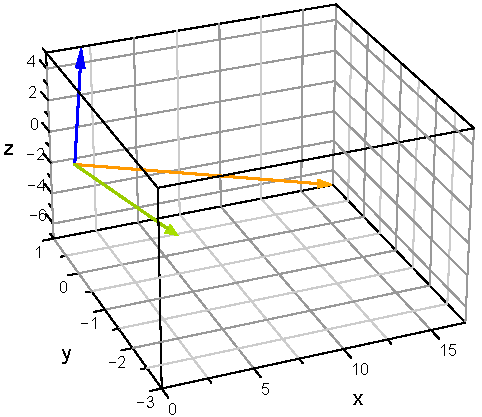
\includegraphics[width=0.5\linewidth]{mai_fig025.pdf}
    \captionof{figure}[Ortogonální doplněk]{Vizualizace vektorového prostoru a jeho    
             ortogonálního doplňku pomocí sw MatLab - MuPAD příkazem:\newline
             \texttt{plot(plot::Arrow3d([1,-3,2]), plot::Arrow3d([2,1,5]), 
             plot::Arrow3d([17,1,-7]))}}
    \label{LA:fig_ort01}
    \par}
\end{example}

      %---------------------------------------------------------------

      Výsledek předchozího příkladu \ref{mai:exam011} lze interpretovat tak, že jsme našli všechny 
      vektory, které jsou kolmé na rovinu určenou vektory ze zadání. Rovina je útvar       
      dvojrozměrný a protože prostor všech vektorů je trojrozměrný, musí nutně mít podprostor 
      ortogonálních vektorů ve shodě se vztahem \ref{LA:eq_dim_doplnek} pouze jednu dimenzi. Vše 
      je dobře patrné z obr. \ref{LA:fig_ort01}

  %=========================== Kapitola: Vlastní čísla a vlastní vektory ==========================
  \section{Vlastní čísla a vlastní vektory}
    \subsection{Motivace} 
      \textbf{Poznámka}: Je-li \(\mathcal{A} : \mathcal{V} \rightarrow \mathcal{V}\) lineární 
      zobrazení z prostoru \(\mathcal{V}\) do prostoru \(\mathcal{V}\) (nikdy se takové zobrazení 
      nazývá lineárním operátorem), pak je přirozeným požadavkem najít takovou bázi prostoru 
      \(\mathcal{V}\), že je matice zobrazení $\mathbf{A}$ v této bázi co nejjednodušší, např. má 
      následující strukturu
      \begin{equation*}
         \mathbf{A}=
           \left(\begin{array}{ccccc}
             \boxed{A_1}       &             &       &       & 0   \\
                 & \boxed{A_2} &             &       &             \\
                 &             & \boxed{A_3} &       &             \\
                 &             &             &\ddots &             \\
              0  &             &             &       & \boxed{A_k}
            \end{array}
           \right),
     \end{equation*}
     kde \(A_k\) jsou čtvercové matice malého řádu (nejlépe \(1\) nebo \(2\)) a ostatní prvky 
     matice jsou nulové. Problém najít bázi, aby v ní matice zobrazení měla diagonální tvar (kde 
     \(A_k\) jsou skaláry), vede k pojmu vlastní číslo a vlastní vektor matice.

      \begin{definition} 
        Nechť \(\mathbf{A}\in \mathcal{C}^{n,n}\) (matice je čtvercová řádu \(n\)).
        \begin{equation}
          \mathbf{A} = (a_{ij}) =
            \begin{pmatrix}
              a_{11} & a_{12} & \ldots & a_{1n} \\
              a_{21} & a_{22} & \ldots & a_{2n} \\
              \vdots & \vdots & \ddots & \vdots \\
              a_{n1} & a_{n2} & \ldots & a_{nn}
            \end{pmatrix}
        \end{equation}

        Jestliže platí
        \begin{equation}\label{eq:vl_number}
          \mathbf{Au} = \lambda\mathbf{u}
        \end{equation}
        pro jisté komplexní číslo \(\lambda\in\mathcal{C}\)  a jistý nenulový vektor 
        \(x\in\mathcal{C}^n, \mathbf{u}\neq\Theta\), potom číslo \(\lambda\) nazýváme 
        \textbf{vlastním číslem} matice \(\mathbf{A}\) a vektor \(\mathbf{u}\) \textbf{vlastním 
        vektorem} příslušným k tomuto vlastnímu číslu. Množinu všech vlastních čísel nazýváme 
        \textbf{spektrem matice} \(\mathbf{A}\). Pokud rov. \ref{eq:vl_number} rozepíšeme, dostaneme
        \begin{equation}
          \begin{pmatrix}
            a_{11} & a_{12} & \ldots & a_{1n} \\
            a_{21} & a_{22} & \ldots & a_{2n} \\
            \vdots & \vdots & \ddots & \vdots \\
            a_{n1} & a_{n2} & \ldots & a_{nn}
          \end{pmatrix}   \cdot
          \begin{pmatrix}
            u_{1} \\  u_{2} \\ \vdots \\  u_{n} \\
          \end{pmatrix}    =\lambda\cdot
          \begin{pmatrix}
            u_{1} \\ u_{2} \\ \vdots \\ u_{n} \\
          \end{pmatrix}
        \end{equation}
        můžeme ji rovněž psát ve tvaru
        \begin{equation*}
            \begin{pmatrix}
            \setlength{\arraycolsep}{3pt}
              a_{11} -\lambda & a_{12}           & \ldots & a_{1n} \\
              a_{21}          & a_{22} -\lambda  & \ldots & a_{2n} \\
              \vdots          & \vdots           & \ddots & \vdots \\
              a_{n1}          & a_{n2}           & \ldots & a_{nn}-\lambda
            \end{pmatrix} \cdot
          \begin{pmatrix}
            u_{1} \\ u_{2} \\ \vdots \\ u_{n} \\
          \end{pmatrix}  =
          \begin{pmatrix}
              0 \\ 0 \\ \vdots \\ 0 \\
            \end{pmatrix}
        \end{equation*}
      \end{definition}

       Tato soustava rov. je \textbf{homogenní} a stručně ji můžeme zapsat
      \begin{equation}\label{vv_hom_zapis}
        \left(\mathbf{A} - \lambda\mathbf{I}\right) = \mathbf{0}
      \end{equation}
      Homogenní soustava má \emph{netriviální řešení}, právě když je determinant matice soustavy 
      roven  nule, tj. v případě soustavy rov. rov. \ref{vv_hom_zapis} platí
      \begin{equation}\label{vv_hom_reseni}
        \abs{\mathbf{A} - \lambda\mathbf{I}} = \mathbf{0}
      \end{equation}
      Determinant \(A(\lambda)=\abs{\mathbf{A} - \lambda \mathbf{I}}\) nazýváme 
      \textbf{charakteristický polynom} matice \(\mathbf{A}\) - jedná se o polynom stupně \(n\) v 
      proměnné \(\lambda\), který má v oboru komplexních čísel \(n\) kořenů. Rovnici 
      \(A(\lambda)=0\) nazýváme \textbf{charakteristická rovnice matice \(\mathbf{A}\)} - jejími 
      kořeny jsou \textbf{charakteristické hodnoty} (resp. \textbf{vlastní čísla}) 
      \textbf{matice} \(\mathbf{A}\).
            
      \begin{note}
        U vlastních čísel studium pouze reálných matic ztrácí smysl, protože i 
        reálná matice může mít komplexní vlastní čísla. Proto se uvažuje obecná komplexní matice.
      \end{note}
      
      \begin{note}
        Podmínka existence nenulového vektoru \(\mathbf{u} = \Theta\) v definici 
        vlastního čísla je nezbytná: kdyby bylo připuštěno i \(\mathbf{u} = \emptyset\), potom by 
        každé komplexní číslo bylo vlastním číslem a definice by ztratila smysl.
      \end{note}
      
      \begin{note}
        Odpovídá-li matice \(\mathbf{A}\) matici nějakého zobrazení \(\mathcal{A}\), pak každý 
        nenulový vektor z jádra zobrazení \(\ker\mathcal{A}\) je vlastním vektorem příslušným 
        vlastnímu číslu \(\lambda\). Je-li \(\ker\mathcal{A} = \{\Theta\}\) 
        (je-li matice \(\mathbf{A}\) regulární), pak \(\Theta\) není vlastním číslem matice 
        \(\mathbf{A}\).
      \end{note}

      %---------------------------------------------------------------
        % !TeX spellcheck = cs_CZ
\begin{mathexam}{Ortogonální projekce v prostoru \(\mathcal{R}^3\)}{exam012}
    Je-li \(\mathbf{P}\) matice ortogonální projekce v prostoru \(\mathcal{R}^3\) na nějaký 
    podprostor \(\mathcal{U}\) (\(\mathcal{U}\) je tedy buď rovina nebo přímka procházející 
    počátkem), pak pro každý vektor \(\mathbf{u}\in\mathcal{U}\) platí \(\mathbf{Pu} = 
    \mathbf{u}\), všechny vektory z \(\mathcal{U}\) (s výjimkou nulového vektoru \(\Theta\)) 
    jsou vlastními vektory matice $\mathbf{P}$ příslušné vlastnímu číslu \(\lambda\). Prostor 
    \(\mathrm{U}^\bot\) je roven jádru projekce (nulovému prostoru matice \(\mathbf{P}\)), 
    a tedy každý vektor z ortogonálního doplňku \(\mathcal{U}\) (s výjimkou \(\Theta\)) je 
    vlastním vektorem příslušným k vlastnímu číslu \(0\).

    {\centering
      \captionsetup{type=figure}
      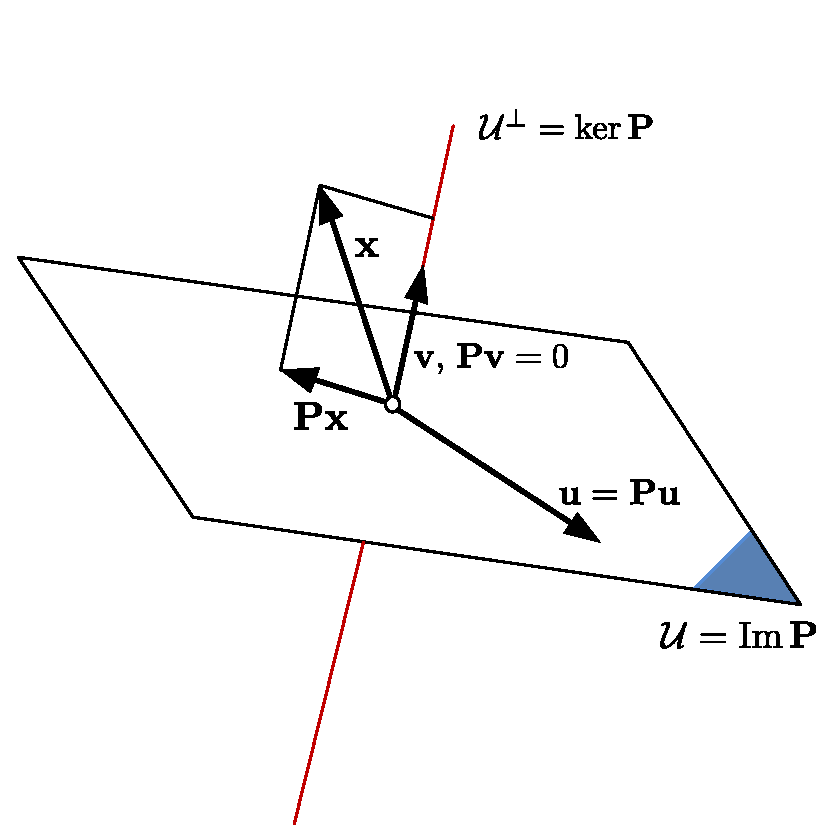
\includegraphics[width=0.5\linewidth]{mai_fig024.pdf}
      \captionof{figure}{K příkladu \ref{mai:exam012}}
      \label{mai:FIG016}
      \par}

\end{mathexam}
      %---------------------------------------------------------------

      %---------------------------------------------------------------
        % !TeX spellcheck = cs_CZ
\begin{mathexam}{Určete spektrum matice a její spektrální poloměr následující matice
  \begin{equation*}\label{pr:spektrum_matice}
    \mathbf{A} =
      \begin{pmatrix}
        2  &        2    & 0 \\
       -3  &       -3    & 5 \\
        0  & -\num{0.25} & 2
      \end{pmatrix}
  \end{equation*}
  }{exam013} 
  \textbf{Řešení}: Spektrum matice je množina všech jejích vlastních čísel. Spektrální poloměr je
  maximum z absolutních hodnot vlastních čísel. Vlastní čísla určíme z charakteristické rovnice
  \(\det(\mathbf{A}-\lambda \mathbf{I})=0\).
      \begin{equation*}
        \textbf{A} - \lambda\textbf{I}=
          \begin{pmatrix}
            2-\lambda  &  2          & 0 \\
           -3          & -3-\lambda  & 5 \\
            0          & -0.25       & 2-\lambda
        \end{pmatrix}
      \end{equation*}
      \begin{align}
        \det(\mathbf{A}-\lambda \mathbf{I})                    &= 0           \nonumber\\
        (2-\lambda)
          \begin{pmatrix}
            -3-\lambda  &  5\\
              -0.25    &  2 - \lambda
          \end{pmatrix} -2\cdot
          \begin{pmatrix}
            -3       &  5\\
            0       &  2 - \lambda
          \end{pmatrix}                                        &= 0           \nonumber\\
        (2-\lambda)^2(-3-\lambda)+1.25(2-\lambda)+6(2-\lambda) &= 0           \nonumber\\
        (2-\lambda)[(2-\lambda)(-3-\lambda)+1.25+6]            &= 0           \nonumber\\
        (2-\lambda)(\lambda^2+\lambda+1.25)                    &= 0           \nonumber
      \end{align}
      \begin{equation*}
        \lambda_1 = 2, \quad\lambda_2 = -0.5+i, \quad\lambda_3=-0.5-i
      \end{equation*}
      \begin{itemize}
        \item Spektrum matice \(\mathbf{A}\) je \(\sigma(\mathbf{A})=\{2,-0.5+i,-0.5-i\}\).
        \item Spektrální poloměr \(\rho(\mathbf{A})=\max_i\abs{\lambda_i}=2\).
      \end{itemize}

  %    \attachfile[icon=Paperclip, description=Matlab Determine the spectrum of a matrix 
  %      and its spectral radius]{../SRC/MAI/matlab/LA001.m}
\end{mathexam}
      %---------------------------------------------------------------

      %---------------------------------------------------------------
        % !TeX spellcheck = cs_CZ
\begin{mdframed}[style=mdexam]
  \begin{example}\label{mai:exam014}
    Určete vlastní čísla a vlastní vektory matice \(\mathbf{B} = \mathbf{A}^2 - 4\mathbf{A} + 
    9\mathbf{A}^{-1} - \mathbf{I}\), kde \(\mathbf{A}\) je matice \(\mathbf{A}= 
    \begin{pmatrix}1&0.5\\3.5&4\end{pmatrix}\).

    \textbf{Řešení}: (z předchozího příkladu víme, že \(\lambda_1=4.5, \lambda_2=0.5\)) a
    \(\mathbf{I}\) jednotková matice. Označme symbolem \(\lambda\) vlastní číslo matice 
    \(\mathbf{A}\) a nechť \(\mathbf{x}\) je příslušný vlastní vektor. Pak platí:
    \begin{itemize}
      \item Matice \(\mathbf{A}^2\) má vlastní čísla rovna \(\lambda^2\).
      \item Matice \(4\mathbf{A}\) má vlastní čísla rovna \(4\lambda\).
      \item Matice \(9\mathbf{A}^{-1}\) má vlastní čísla rovna \(\frac{9}{\lambda}\).
    \end{itemize}
    Matice \(\mathbf{B}=\mathbf{A}^2-4\mathbf{A}+9\mathbf{A}^{-1}-\mathbf{I}\) má vlastní čísla 
    ve tvaru  \(\lambda^2-4\lambda+\frac{9}{\lambda}-1\), vlastní vektory jsou stejné jako 
    vlastní vektory odpovídající vlastním číslům matice \(\mathbf{A}\). Tedy:
    \begin{multline*}
        \sigma(B)=\{4.5^2-4\cdot4.5+\frac{9}{4.5}-1,\\
        0.5^2-4\cdot0.5+\frac{9}{0.5}-1\}=\{3.25, 15.25\}
    \end{multline*}
  \end{example}
\end{mdframed}
      %---------------------------------------------------------------


      %---------------------------------------------------------------
       % !TeX spellcheck = cs_CZ
\begin{mahtexam}{Určete vlastní čísla a odpovídající vlastní vektory následují\-cích matic:
  \begin{equation*}
    \mathbf{A}=
      \begin{pmatrix}
        1   & 0.5\\
        3.5 & 4
      \end{pmatrix}, \quad
    \mathbf{B}=
      \begin{pmatrix}
        3   & -1 \\
        2.5 &  4 
      \end{pmatrix}
  \end{equation*}
  }{exam002}

  Vlastní čísla určíme z charakteristické rovnice: \(\det(\mathbf{A} - \lambda\mathbf{I}) = 0\).
  Vlastní vektory \(\mathbf{x_i}\) odpovídající vlastním číslům \(\lambda_i\), jsou řešením
  homogenní soustavy rovnic \((\mathbf{A} - \lambda_i\mathbf{I})\mathbf{x_i} = 0\).
  \begin{itemize}
    \item Vlastní čísla matice \textbf{A}:
      \begin{equation*}
          \textbf{A} - \lambda\textbf{I} =
            \begin{pmatrix}
                1-\lambda  &  0.5          \\
              -3.5         &  4-\lambda
            \end{pmatrix}
      \end{equation*}
      \begin{align*}
        \det(\mathbf{A}-\lambda\mathbf{I}) &= 0 \\
        (1-\lambda)(4-\lambda)-\frac{7}{4} &= 0 \\
        \lambda^2-5\lambda+\frac{9}{4}     &= 0
      \end{align*}
      \begin{equation*}
        \lambda_1 = 4.5,\quad \lambda_2 = 0.5
      \end{equation*}
  \end{itemize}

  \begin{itemize}
    \item Vlastní čísla matice \textbf{B}:
      \begin{equation*}
          \textbf{B} - \lambda\textbf{I}=
            \begin{pmatrix}
              3-\lambda  & -1             \\
              2.5        &  4-\lambda
            \end{pmatrix}
      \end{equation*}
      \begin{align*}
        \det(\mathbf{B}-\lambda\mathbf{I}) &= 0 \\
        (3-\lambda)(4-\lambda)+\frac{5}{2} &= 0 \\
        \lambda^2-7\lambda+\frac{29}{2}    &= 0
      \end{align*}
      \begin{equation*}
        \lambda_1 = \frac{7+3i}{2},\quad \lambda_2 = \frac{7-3i}{2}
      \end{equation*}
  \end{itemize}
  % matice A
  Vlastní vektor matice \(\mathbf{A}\) pro \(\lambda_1=4.5: (\mathbf{A} -
  \lambda_1\mathbf{I})\mathbf{x_1} = 0 \Rightarrow\)
  \begin{equation*}
    \begin{pmatrix}
      1  -4.5  &  0.5     \\
      -3.5     &  4-4.5
    \end{pmatrix}
    \sim
    \begin{pmatrix}
      -3.5  &  0.5         \\
      -3.5  & -0.5
    \end{pmatrix}
  \end{equation*}
  \begin{equation*}
    \Rightarrow\mathbf{x_1} =
    \begin{pmatrix}
      1 \\ 7
    \end{pmatrix}
    \, r, r\in\mathbb{R}, r\neq0
  \end{equation*}
  Vlastní vektor matice \(\mathbf{A}\) pro \(\lambda_2=0.5: (\mathbf{A} -
  \lambda_1\mathbf{I})\mathbf{x_2}=0 \Rightarrow\)
  \begin{equation*}
    \begin{pmatrix}
      1  -0.5  &  0.5   \\
      -3.5      &  4-0.5
    \end{pmatrix}
    \sim
    \begin{pmatrix}
      0.5  &  0.5       \\
      3.5  &  3.5
    \end{pmatrix}
  \end{equation*}
  \begin{equation*}
    \Rightarrow\mathbf{x_2} =
    \begin{pmatrix}
      -1 \\ 1
    \end{pmatrix}
    \, r, r\in\mathbb{R}, r\neq0
  \end{equation*}
  % matice B
  Vlastní vektor matice \(\mathbf{A}\) pro \(\lambda_1=\frac{7+3i}{2}: (\mathbf{B} -
  \lambda_1\mathbf{I})\mathbf{x_1}=0 \Rightarrow\)
  \begin{align*}
    \begin{pmatrix}
      3 - \frac{7+3i}{2}            & -1                                       \\
      \frac{5}{2}                   &  4 - \frac{7+3i}{2}
    \end{pmatrix}
    &\sim
    \begin{pmatrix}
      -\frac{1}{2}-\frac{3}{2}i      &  -1                                     \\
      \frac{5}{2}                    & \frac{1}{2}-\frac{3}{2}i
    \end{pmatrix}
    \sim                                                                            \\
    \begin{pmatrix}
      -\frac{10}{4}                  &-\left(\frac{1}{2} -\frac{3}{2}i\right)  \\
      \frac{5}{2}                    & \frac{1}{2}-\frac{3}{2}i
    \end{pmatrix}
    &\sim
    \begin{pmatrix}
      -5                           &-\left(1-3i\right)                         \\
        5                           & \left(1-3i\right)
    \end{pmatrix}
  \end{align*} 
  \begin{align*} 
    \Rightarrow \mathbf{x_1}=
    \begin{pmatrix}
      -1+3i \\ 5
    \end{pmatrix}
    \, r, r\in\mathbb{C}, r\neq0
  \end{align*}
  Vlastní vektor matice \(\mathbf{B}\) pro \(\lambda_2=\frac{7-3i}{2}: (\mathbf{B} -
  \lambda_1\mathbf{I})\mathbf{x_2}=0 \Rightarrow\)
  \begin{align*}
    \begin{pmatrix}
      3  - \frac{7-3i}{2}       &  -1                                     \\
      \frac{5}{2}               &  4 - \frac{7-3i}{2}
    \end{pmatrix}
    &\sim
    \begin{pmatrix}
      -\frac{1}{2}+\frac{3}{2}i  &  -1                                     \\
      \frac{5}{2}                & \frac{1}{2}+\frac{3}{2}i
    \end{pmatrix}                                 
    \sim                                                                          \\
    \begin{pmatrix}
      -\frac{10}{4}              &-\left(\frac{1}{2} +\frac{3}{2}i\right)  \\
      \frac{5}{2}                & \quad\frac{1}{2}+\frac{3}{2}i
    \end{pmatrix}
    &\sim                                                                   
    \begin{pmatrix}
      -5                         &-\left(1+3i\right)                       \\
      5                          & \quad\left(1+3i\right)
    \end{pmatrix}
  \end{align*} 
  \begin{equation*} 
    \Rightarrow \mathbf{x_2}=
    \begin{pmatrix}
      -1-3i \\ 5
    \end{pmatrix}
    \, r, r\in\mathbb{C}, r\neq0
  \end{equation*}
  %---------------------------------------------------------------
  \lstinputlisting[%
    style=luaMatlabStyle,
    caption={Výpis programu pro ověření výpočtu vlastních čísel matic programem Matlab.}
    ]{../src/MAI/matlab/LA001.m}
  %--------------------------------------------------------------- 
\end{mathexam}
      %---------------------------------------------------------------


%---------------------------------------------------------------------------------------------------